\documentclass[10pt]{beamer}

\usepackage{verbatim}
\usepackage{graphicx,color}
\usepackage{xspace}
\usepackage{tikz}
\usepackage{url}

\usecolortheme{rose}
\setbeamertemplate{footline}{}
\setbeamertemplate{navigation symbols}{}
\setbeamercovered{invisible}
 
\usepackage{fontspec}

\setsansfont{PalatinoSansLTPro}[
   Path = /home/charles/charles_work/fonts/PalatinoSans/, 
   Extension      = .otf,
   UprightFont    = *-Regular,
   BoldFont= *-Bold ,
   ItalicFont = *-Italic,
   BoldItalicFont = *-BoldIta
]





\subtitle{Organisation}
\author[C. Bouillaguet]{\textbf{Charles Bouillaguet / Vincent Neiger}}
\institute[SU]{Sorbonne Université}

\date{PPAR}

\begin{document}
%\maketitle

\begin{frame}
  
  \centering

  \scalebox{6}{\bfseries \alert{Welcome !}}
  
  \vspace{1cm}
  
  \textbf{\Large Parallel Programming (PPAR)}

  \bigskip

  a.k.a. MU4I903 (university masters) a.k.a. N8-IPA (MAIN4)
\end{frame}

%%%%%%%%%%%%%%%%%%%%%%%%%%%%%%%%%%%%%%%%%%%%%%%%%%%%%%%%%%%%%%%%%%%%%%%%%%%%%%%%%

\begin{frame}
  \frametitle{This is the Boring Part}

  \begin{block}{Documents, Planning, etc.}
    Everything is on Moodle !!
  \end{block}
  
  \begin{itemize}
  \item 10 weeks
  \item 1 week = lecture + TD (exercises) + TP (hands-on in lab room)
  \item TP: you have to submit (brief) reports on Moodle (``homework'')
  \item No midterm exam (``partiel'')
  \item Final exam in January (January 11th?)
  \item Two projects (medium to high difficulty ; lots of work)
    \begin{itemize}
    \item Deadline \#1: November 11th
    \item Deadline \#2: January 11th (tentative)
    \end{itemize}
  \end{itemize}
\end{frame}

%%%%%%%%%%%%%%%%%%%%%%%%%%%%%%%%%%%%%%%%%%%%%%%%%%%%%%%%%%%%%%%%%%%%%%%

\begin{frame}
  \begin{block}{How Will You be Evaluated?}
    \begin{itemize}
    \item \textbf{Final Exam (20 points)} 
      \begin{itemize}
      \item Actual date unknown (educated guess: January 11th)
      \end{itemize}

      \medskip
      
    \item \textbf{Two projects (2 $\times$ 20 points)} 
      \begin{itemize}
      \item November 11th
      \item January 10th (?)
      \end{itemize}
      
      \medskip

    \item \textbf{Homework (0 points)} 
      \begin{itemize}
      \item Not graded but you'll be punished if you don't return it
      \end{itemize}
    \end{itemize}
  \end{block}

  \begin{alertblock}{Course Validation Recipe}
    \begin{itemize}
    \item Final grade $\geq$ 30 $\Longrightarrow$ you pass. Bye-bye!
    \item Otherwise:
      \begin{itemize}
      \item You take another written exam in June (20 points)
      \item It replaces your worst earlier grade
      \item New final grade $\geq$ 30 $\Longrightarrow$ you pass
      \end{itemize}
    \end{itemize}
  \end{alertblock}
\end{frame}

%%%%%%%%%%%%%%%%%%%%%%%%%%%%%%%%%%%%%%%%%%%%%%%%%%%%

\begin{frame}
  \frametitle{Prerequisites for this Class}
  \begin{block}{Just two (but they are important)}
    \begin{itemize}
    \item<2-> You know how to code in C
    \item<3-> You know how to use a terminal and the shell
    \end{itemize}
  \end{block}
  
  \begin{overlayarea}{\textwidth}{4cm}
    \begin{columns}
      \begin{column}{0.47\textwidth}
        \includegraphics<2->[width=\textwidth]{tc.png}
      \end{column}
      \begin{column}{0.47\textwidth}
        \includegraphics<3->[width=\textwidth]{terminal.jpg}
      \end{column}
    \end{columns}
  \end{overlayarea}
  
  \begin{alertblock}<4->{Just in case}
    If you're not fluent with the C language, come talk to me at the end
  \end{alertblock}
\end{frame}

%%%%%%%%%%%%%%%%%%%%%%%%%%%%%%%%%%%%%%%%%%%%%%%%%%%

\begin{frame}
  \begin{block}{Why the C language?}
  \begin{itemize}
  \item 99.9\% of (serious) scientific computing is in Fortran / C / C++

    \medskip

  \item C / Fortran are \textbf{mature} and \textbf{stable}
    \begin{itemize}
    \item Fortran (resp. C) started in 1955 (resp. 1972)
    \item Code from 50 years ago compiles and works fine
    \item Fortran libraries from the late 1970's still used today!
    \end{itemize}

    \medskip

  \item There is \textbf{always} a C compiler
    \begin{itemize}
    \item Even on the most exotic HPC platform
    \end{itemize}    
  \end{itemize}
\end{block}

\begin{exampleblock}{Here comes a new challenger: Python is \textbf{gaining traction}}
  \begin{itemize}
  \item \textbf{Not mature yet} (code from $\leq$ 10 years ago \alert{no longer runs})
  \item \textbf{Interpreted} language ($\approx 1000\times$ \alert{slower} than C / Fortran)
  \item Python packages used in scientific computing (\texttt{numpy}, \texttt{scipy}, ...)
    \begin{itemize}
    \item ... are just \emph{wrappers} around C / Fortran code that do the heavy lifting
    \end{itemize}
  \end{itemize}
\end{exampleblock}
\end{frame}

%%%%%%%%%%%%%%%%%%%%%%%%%%%%%%%%%%%%%%%%%%%%%%%%%%%

\begin{frame}
  \frametitle{Course Material}

  \begin{itemize}
  \item All${}^1$ the course materials (\texttt{.pdf} files) are${}^2$ available on Moodle
  \item Public domain
  \item \LaTeX sources available
    \begin{center}
      \url{https://github.com/cbouilla/PPAR}
    \end{center}

    \medskip

  \item If you find a typo/error/misspell/etc., \textbf{please}
    \begin{itemize}
    \item Open a github issue
    \item Even better, fix it and send a pull request
    \end{itemize}
  \end{itemize}

  \vfill

  \tiny
  \begin{enumerate}
  \item The TD/TP handouts are not there yet because our files contain the answers. We are working on it
  \item or they will be at some point
  \end{enumerate}
\end{frame}

%%%%%%%%%%%%%%%%%%%%%%%%%%%%%%%%%%%%%%%%%%%%%%%%%%%%

\begin{frame}
  \frametitle{Programming is \textbf{not} a science}

  \centering
  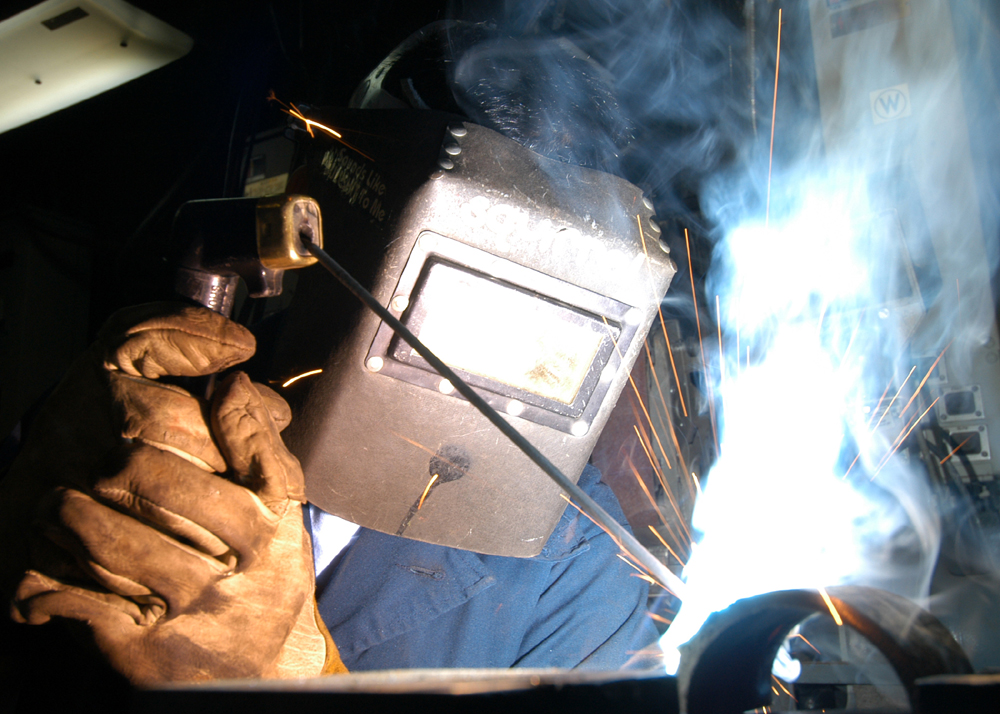
\includegraphics[width=\textwidth]{welding.jpg}
\end{frame}

%%%%%%%%%%%%%%%%%%%%%%%%%%%%%%%%%%%%%%%%%%%%%%%%%%%% 

\begin{frame}
  \frametitle{Programming is \textbf{not} a science}

  \centering
  
\includegraphics[width=\textwidth]{maison.jpg}
\end{frame}

%%%%%%%%%%%%%%%%%%%%%%%%%%%%%%%%%%%%%%%%%%%%%%%%%%%% 

\begin{frame}
  \frametitle{Programming is \textbf{not} a science}

  \centering
  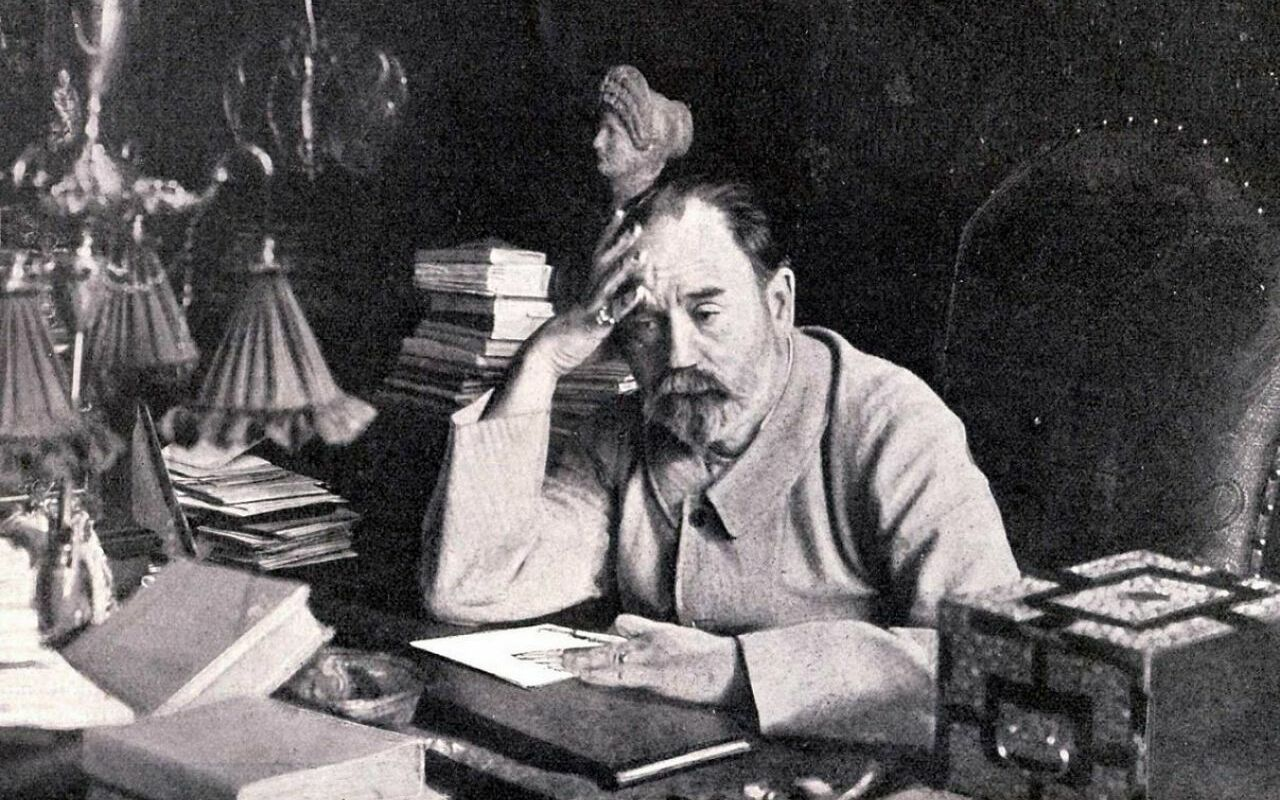
\includegraphics[width=\textwidth]{zola.jpg}
\end{frame}

%%%%%%%%%%%%%%%%%%%%%%%%%%%%%%%%%%%%%%%%%%%%%%%%%%%% 

\begin{frame}
  \frametitle{\textbf{Practice} is the only way}
  \framesubtitle{$\Rightarrow$ Two heavy projects \raisebox{-2pt}{\includegraphics[height=\baselineskip]{content.png}}}
  \begin{block}{Course Project\textbf{s}}
    \begin{itemize}
      
    \item \textbf{Concept} :
      \begin{itemize}
      \item We provide you with some \textbf{sequential} code
      \item You have to \textbf{parallelize} it
      \item Evaluate the \textbf{performance} of your work
      \item Run it on \textbf{challenging inputs} (using lots of cores)
      \item Write a \textbf{report} about what happened
      \end{itemize}
  
      \medskip

    \item They are \textbf{not easy} and require a \textbf{non-trivial amount of work} \includegraphics[width=0.5cm,trim=0 17mm 0 0]{triste}
      
      \medskip
      
    \item Starting 2 days before the deadline is the recipe for \textbf{disaster}
      \begin{itemize}
      \item We keep telling you but it unfortunately happens every year...
      \end{itemize}
    \end{itemize}
  \end{block} 
\end{frame}

%%%%%%%%%%%%%%%%%%%%%%%%%%%%%%%%%%%%%%%%%%%%%%%%%%%%

{
  \setbeamercolor{background canvas}{bg=black}
\begin{frame}
  \frametitle{\color{white} We are going to \textbf{make you} learn...}
  \framesubtitle{\color{white} Teaching staff \#1: Charles Bouillaguet}
  
  \centering
  
\includegraphics[height=8cm]{severus.jpg}
\end{frame}
}

%%%%%%%%%%%%%%%%%%%%%%%%%%%%%%%%%%%%%%%%%%%%%%%%%%%%% 

{
  \setbeamercolor{background canvas}{bg=black}
\begin{frame}
  \frametitle{\color{white} ...the \textbf{hard} way}
  \framesubtitle{\color{white} Teaching staff \#2: Vincent Neiger}

  \centering
  
\includegraphics[height=7.5cm]{gto.jpg}
\end{frame}
}

%%%%%%%%%%%%%%%%%%%%%%%%%%%%%%%%%%%%%%%%%%%%%%%%%%%%%%%%

\begin{frame}[label=tme]
  \frametitle{Computing Infrastructure}

  \begin{columns}
    \begin{column}{7cm}

      \begin{block}{\textbf{Practice} parallel programming}
        \begin{itemize}
        \item Need parallel machines...
        \item No serious infrastructure @ SU
          \begin{itemize}
          \item (there is some but not for students \raisebox{-2pt}{\includegraphics[height=\baselineskip]{triste.png}}
)
          \end{itemize}
        \end{itemize}
      \end{block}

      \medskip

      \begin{center}
        
\includegraphics{grid5000_logo.png}
      \end{center}
      
      \begin{exampleblock}{We'll use grid5000 (aka g5K)}
        \begin{itemize}
        \item Decent approximation of a real computing center
        \end{itemize}
      \end{exampleblock}
      
    \end{column}
    \begin{column}{4cm}
    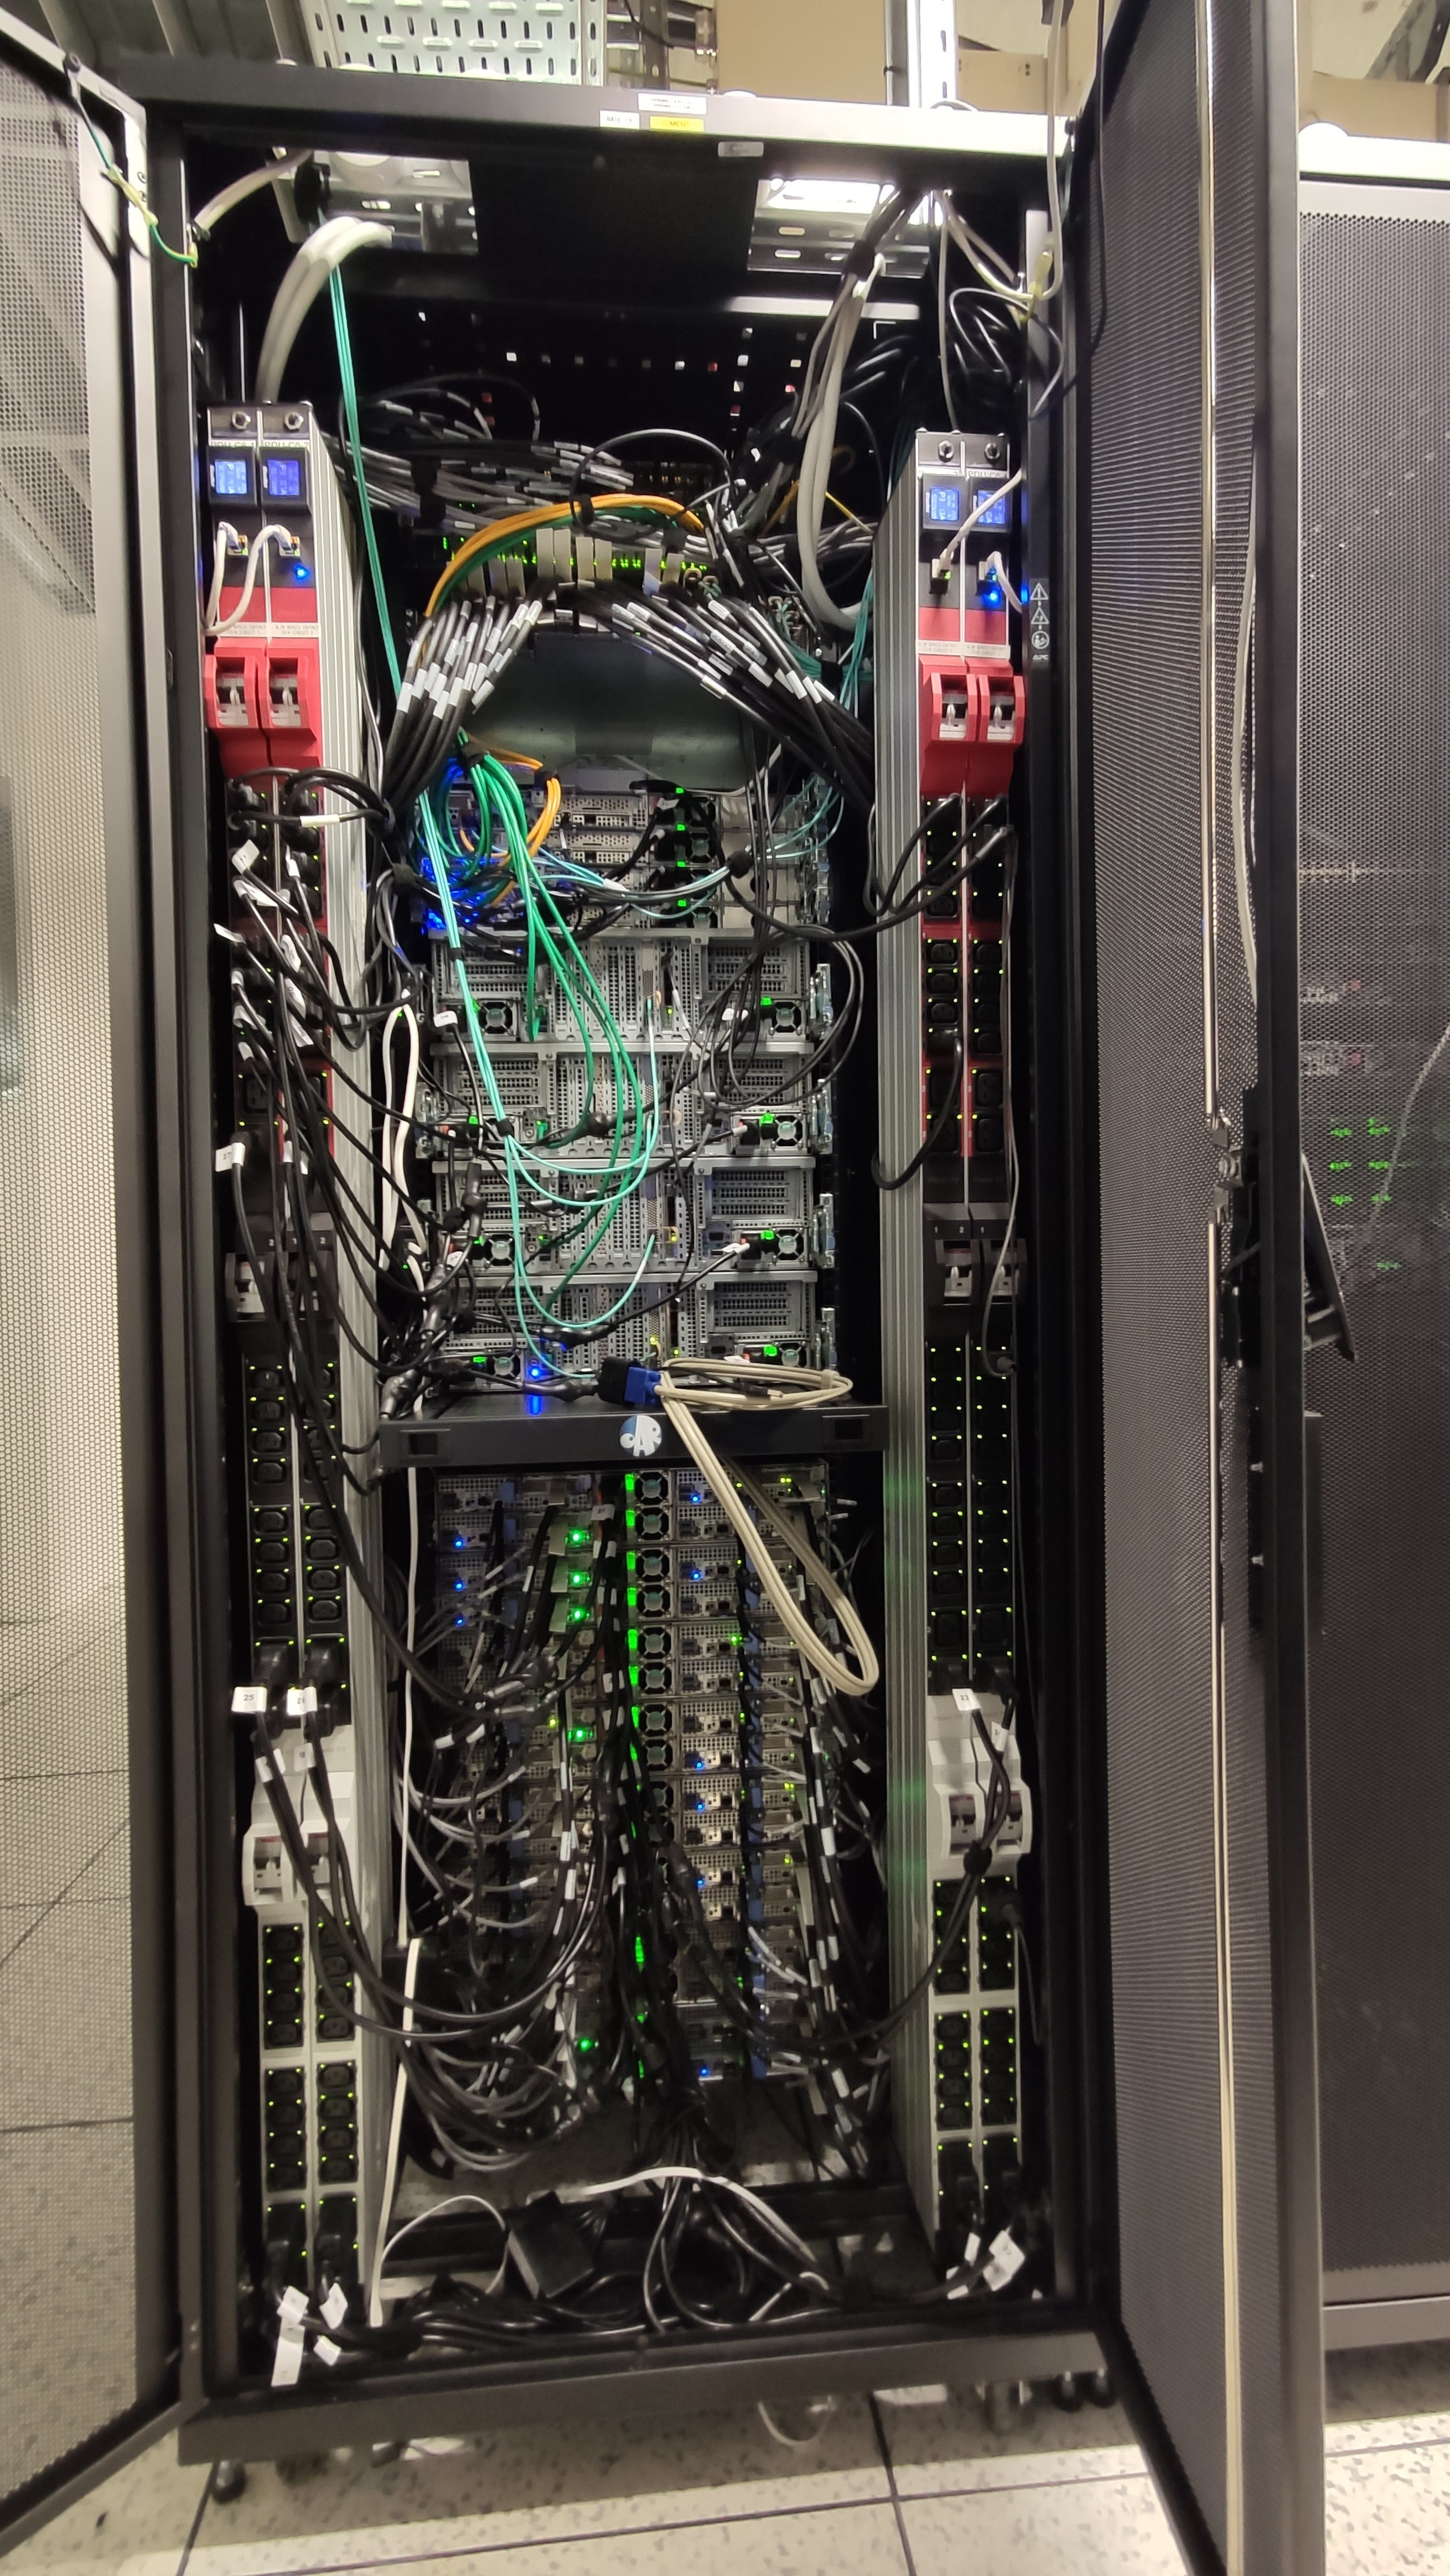
\includegraphics[height=8cm]{cluster.jpg}
  \end{column}
\end{columns}
\end{frame}

%%%%%%%%%%%%%%%%%%%%%%%%%%%%%%%%%%%%%%%%%%%%%%%%%%%%%

\begin{frame}[label=tme]
  
\includegraphics{grid5000_logo.png}

  \begin{columns}
    \begin{column}{5cm}

      \begin{exampleblock}{What is it?}
        \begin{itemize}
        \item Experimental research platform 
        \item Mutualized computing resources
        \end{itemize}
      \end{exampleblock}
      
      \begin{block}{Concretely}
        \begin{itemize}
        \item 8 geographic sites
        \item 37 clusters
        \item 806 ``computers''
        \item 15,702 CPU cores
        \end{itemize}
      \end{block}

      %%%%%%%%%%%%
      
    \end{column}
    \begin{column}{7cm}
      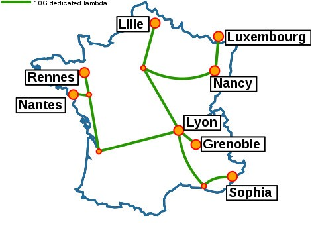
\includegraphics[width=7cm]{grid5000.pdf}
    \end{column}
  \end{columns}
\end{frame}

% %%%%%%%%%%%%%%%%%%%%%%%%%%%%%%%%%%%%%%%%%%%%%%%%%%%%%

% \begin{frame}[label=tme]
%   \frametitle{
\includegraphics[height=1cm]{grid5000_logo.png}}

%   \begin{block}{Accès à distance via \textbf{ssh}}
%     \begin{enumerate}
%     \item Connection à un \textbf{serveur d'accès} de Grid'5000
%       \begin{itemize}
%       \item \texttt{ssh login@access.grid5000.fr}
%       \end{itemize}

%       \smallskip
      
%     \item Connection à la \textbf{frontale} d'un \textbf{site}
%       \begin{itemize}
%       \item \texttt{ssh nancy}
%       \end{itemize}

%       \smallskip
      
%     \item Réservation des \textbf{noeuds de calcul} via \textbf{OAR}
%       \begin{itemize}
%       \item \texttt{oarsub --interactive --property "cluster='gros'"}
%       \end{itemize}

%       \smallskip
      
%     \item Hop ! Connecté à un noeud de \texttt{gros}
%       \begin{itemize}
%       \item 18 coeurs à 2.2Ghz, 96Go de RAM, 25Gbps ethernet
%       \end{itemize}
%     \end{enumerate}
%   \end{block}

%   \begin{alertblock}{Conditions d'utilisation}
%     \begin{itemize}
%     \item Ne pas monopoliser les ressources
%     \item Ne pas miner de cryptomonnaies (même ``pour la science'')
%     \end{itemize}
%   \end{alertblock}
% \end{frame}

%%%%%%%%%%%%%%%%%%%%%%%%%%%%%%%%%%%%%%%%%%%%%%%%%%%%%

\begin{frame}[label=tme]
  \frametitle{
\includegraphics[height=1cm]{grid5000_logo.png}}

  \begin{exampleblock}{RTFM}
    \begin{itemize}
    \item Read the doc on \url{https://www.grid5000.fr}
    \item Re-read it
    \item Read it again
    \end{itemize}
  \end{exampleblock}
  
  \medskip

  \begin{alertblock}{Usage Policy}
    Free scientific instrument, but there are rules (cf. website)
    \begin{itemize}
    \item Do not monopolize resources \emph{during the day}
      \begin{itemize}
      \item Nights / week-ends: you can do whatever you want
      \end{itemize}
    \item \textbf{NEVER} mine cryptocurrencies (not even ``for science'')
    \end{itemize}
  \end{alertblock}  
\end{frame}

%%%%%%%%%%%%%%%%%%%%%%%%%%%%%%%%%%%%%%%%%%%%%%%%%%%%%%%%%%%%%%%%%%%%%%%%

\begin{frame}
  \frametitle{Computing Centers}

  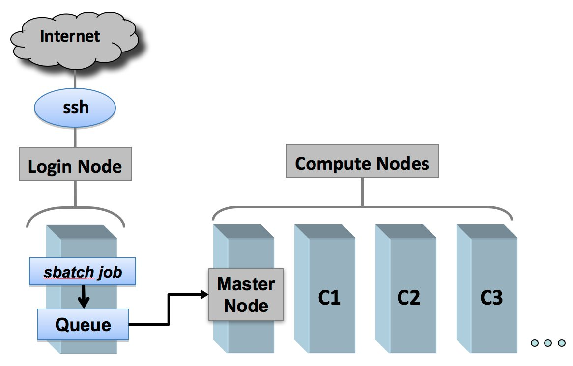
\includegraphics[height=7cm]{compute_center.pdf}
  (image : IDRIS)
  
\end{frame}
 
%%%%%%%%%%%%%%%%%%%%%%%%%%%%%%%%%%%%%%%%%%%%%%%%%%%%%%%%%%%%%%%%%%%%%%%%

\begin{frame}
   \frametitle{Free ad: PRACE Summer of HPC}
   \framesubtitle{PRACE = Partnership for Advanced Computing in Europe}
   \centering
   
\includegraphics[height=8cm]{PRACE_twitter.png}
 \end{frame}
\end{document}

%%% Local Variables:
%%% TeX-command-extra-options: "-shell-escape"
%%% TeX-engine: xetex
%%% End: